% \documentclass[handout]{beamer} % Suppress the pauses to print as handout
\documentclass[aspectratio=169, 11pt]{beamer}
% \documentclass[11pt]{beamer} % Comment the line above and use this line for 4:3 aspect ratio screens
\usepackage{advdate}
\usepackage{amsmath}
\usepackage{amsthm}
\usepackage{amsfonts}
\usepackage{amssymb}
\usepackage{array}
\usepackage{color}
\usepackage{graphicx}
\usepackage{helvet}
\usepackage{hyperref}
\usepackage{mathpazo}
\usepackage{multirow}

\usetheme{CambridgeUS}
\usecolortheme{dolphin}
\usefonttheme[onlymath]{serif}

% Define colors considering color blindness
% Use MATLAB default color palette
\definecolor{blue}{rgb}{0, 0.447, 0.741}
\definecolor{red}{rgb}{0.85, 0.325, 0.098}
\definecolor{yellow}{rgb}{0.929, 0.694, 0.125}
\definecolor{purple}{rgb}{0.494, 0.184, 0.556}
\definecolor{green}{rgb}{0.466, 0.674, 0.188}
\definecolor{cyan}{rgb}{0.301, 0.745, 0.933}
\definecolor{magenta}{rgb}{0.635, 0.078, 0.184}
\definecolor{amber}{rgb}{1.0, 0.75, 0.0}

% Self-defined background and frametitle colors
\definecolor{MyBackground}{RGB}{255, 255, 230}
% Uncomment the following line for plain white background
% \definecolor{MyBackground}{RGB}{255, 255, 255}
\setbeamercolor{background canvas}{bg=MyBackground!40}
\setbeamercolor{frametitle}{bg=MyBackground!80}
% Customize word colors
\setbeamercolor{frametitle}{fg=blue}
\setbeamercolor{title}{fg=blue}
\setbeamercolor{itemize item}{fg=blue}
\setbeamercolor{itemize subitem}{fg=blue}
\setbeamercolor{enumerate item}{fg=blue}
\setbeamercolor{enumerate subitem}{fg=blue}
\setbeamercolor{button}{bg=MyBackground,fg=blue}

% Page number on the bottom
\setbeamertemplate{footline}[frame number]
\setbeamerfont{footline}{size=\fontsize{10}{12}\selectfont}
\setbeamercolor{page number in head/foot}{fg=blue}
% No navigation symbols
\setbeamertemplate{navigation symbols}{}
% No headlines
\setbeamertemplate{headline}{}
% Appendix slides don't count
\newcommand{\backupbegin}{
   \newcounter{framenumberappendix}
   \setcounter{framenumberappendix}{\value{framenumber}}
}
\newcommand{\backupend}{
   \addtocounter{framenumberappendix}{-\value{framenumber}}
   \addtocounter{framenumber}{\value{framenumberappendix}}
}
% Add section title at the beginning of each part
\AtBeginSection[]{
  \begin{frame}[noframenumbering, plain]
  \vfill
  \centering
    \begin{beamercolorbox}[sep=8pt, center, shadow=true, rounded=true]{title}
      \usebeamerfont{frametitle}\insertsectionhead\par%
    \end{beamercolorbox}
  \vfill
  \end{frame}
}

% New theorem environments
\newtheorem{thm}{Theorem}
\newtheorem{lem}[thm]{Lemma}
\newtheorem{prop}[thm]{Proposition}

\beamersetuncovermixins{\opaqueness<1>{25}}{\opaqueness<2->{15}}

% Set pause options to be invisible instead of transparent
\setbeamercovered{invisible}

\begin{document}
\title{Lecture 1 \\ Root-finding, Optimization, Numerical Integration}
\author[Wu]{Peifan Wu}
\date{UBC}

\begin{frame}
\titlepage
\end{frame}

\section{Root-finding}
\begin{frame}
\frametitle{Root-finding Problem}
  \begin{itemize}
    \item[--] We are interested in finding $x^{*}$ that satisfies
    \[
      \begin{array}{cc}
      f\left(x\right)=0 & f\text{ }:\text{}\mathbb{R}\to\mathbb{R}\end{array}
    \]
    Or the fixed point problem
    \[
      f(x)=x
    \]
    \bigskip
    \item[--] Methods:
    \begin{itemize}
      \item[--] Bisection method
      \item[--] Newton's method
      \item[--] Quasi-Newton and Broyden's algorithm
    \end{itemize}
  \end{itemize}
\end{frame}

\begin{frame}
\frametitle{Bisection Method}
  \begin{itemize}
    \item[--] Simple and robust for \textcolor{red}{one-dimensional} continuous function on a closed interval
    \bigskip
    \item[--] Suppose $f(x)$ is defined on $[a,b]$ where $f(a)$ and $f(b)$ have opposite signs
    \item[--] e.g., $f(a)<0$ and $f(b)>0$
    \bigskip
    \item[--] By the mean value theorem there exists at least a zero
    \begin{itemize}
      \medskip
      \item[1.] Set $n=1$, $a^{n}=a$, and $b^{n}=b$
      \medskip
      \item[2.] Compute $c^{n}=\frac{a^{n}+b^{n}}{2}$
      \medskip
      \item[3.] If $f(c^{n})<0$ set $a^{n+1}=c^{n}$ and $b^{n+1}=b^{n}$. Otherwise set $b^{n+1}=c^{n}$ and $a^{n+1}=a^{n}$
      \medskip
      \item[4.] Go back to step \textcolor{blue}{2.} until convergence criterion is satisfied
    \end{itemize}
  \end{itemize}
\end{frame}

\begin{frame}
\frametitle{Advantages and Disadvantages of Bisection Method}
  \begin{itemize}
    \item[--] \textcolor{red}{Robust and Stable}: guaranteed to find an approximate solution
    \bigskip
    \item[--] Does not require computation of derivatives: needs continuity but not differentiability
    \bigskip
    \item[--] \textcolor{red}{Slow} because it does not exploit information on the slope of the function
    \bigskip
    \item[--] \textcolor{red}{Cannot be generalized to the multi-dimensional case}
  \end{itemize}
\end{frame}

\begin{frame}
\frametitle{Newton's Method}
  \begin{itemize}
    \item[--] Approximate the function $f$ at point $x^{n}$ in iteration $n$ as
    \[
      f\left(x\right)\approx f\left(x^{n}\right)+f'\left(x^{n}\right)\left(x-x^{n}\right)
    \]
    and update $x$ \textcolor{blue}{as if you were solving for a zero of the approximation}
    \[
      x^{n+1}=x^{n}-\frac{f\left(x^{n}\right)}{f'\left(x^{n}\right)}
    \]
    \bigskip
    \item[--] $f$ must be differentiable
    \bigskip
    \item[--] fast, but \textcolor{red}{unstable} if function changes derivative quickly
  \end{itemize}
\end{frame}

\begin{frame}
\frametitle{Quasi-Newton Method}
  \begin{itemize}
    \item[--] Use the slope of the secant function going through $f\left(x^{n}\right)$ and $f\left(x^{n+1}\right)$
    \bigskip
    \item[--] Iteration scheme becomes
    \[
      x^{n+1}=x^{n}-\left[\frac{x^{n}-x^{n-1}}{f\left(x^{n}\right)-f\left(x^{n-1}\right)}\right]f\left(x^{n}\right)
    \]
    \bigskip
    \item[--] convergence is slower than Newton method
  \end{itemize}
\end{frame}

\begin{frame}
\frametitle{Broyden's Algorithm}
  \begin{itemize}
    \item[--] \textcolor{red}{Multidimensional version} of the univariate quasi-Newton
    \bigskip
    \item[--] Let $\mathbf{f}:\mathbb{R}^{k}\to\mathbb{R}^{k}$, a system of $k$ equations and $k$ unknowns
    \bigskip
    \item[--] Iteration rule is
    \[
      \mathbf{x}^{n+1}=\mathbf{x}^{n}-\left(\mathbf{J}^{n}\right)^{-1}\mathbf{f}\left(\mathbf{x}^{n}\right)
    \]
    where $\mathbf{J}^{n}$ is the Jacobian evaluated at $\mathbf{x}^{n}$
    \bigskip
    \item[--] To avoid computing $\mathbf{J}^{n}$, use $\mathbf{A}^{n}$ given by secant method:
    \[
      \mathbf{A}^{n+1}=\mathbf{A}^{n}+\left[\mathbf{f}\left(\mathbf{x}^{n+1}\right)-\mathbf{f}\left(\mathbf{x}^{n}\right)-\mathbf{A}^{n}\mathbf{d}^{n}\right]\frac{\left(\mathbf{d}^{n}\right)'}{\left(\mathbf{d}^{n}\right)'\mathbf{d}^{n}}
    \]
    where $\mathbf{d}^{n}=\mathbf{x}^{n+1}-\mathbf{x}^{n}$
    \item[--] Guess of $\mathbf{A}^0$: scaled identity matrix
  \end{itemize}
\end{frame}

\section{Optimization}
\begin{frame}
\frametitle{Minimization}
  \begin{itemize}
    \item[--] We describe \textcolor{red}{minimization} problems: to maximize $f$ is to minimize $-f$
    \item[--] Isomorphisms:
    \begin{itemize}
      \item[--] If $f$ is concave then the minimization problem
      \[
        \min_{x\in\left[a,b\right]}f\left(x\right)
      \]
      is equivalent to root-finding on the FOC $f'\left(x\right)=0$
      \medskip
      \item[--] The multivariate root-finding problem
      \begin{align*}
        f^{1}\left(x_{1},x_{2},\ldots,x_{n}\right) & =0\\
        f^{2}\left(x_{1},x_{2},\ldots,x_{n}\right) & =0\\
        \vdots\\
        f^{n}\left(x_{1},x_{2},\ldots,x_{n}\right) & =0
      \end{align*}
      can be restated as a nonlinear least square problem
      \[
        \min_{\left\{ x_{1},x_{2},\ldots,x_{n}\right\} }\sum_{i=1}^{n}f^{i}\left(x_{1},x_{2},\ldots,x_{n}\right)^{2}
      \]
    \end{itemize}
  \end{itemize}
\end{frame}

\begin{frame}
\frametitle{Bracketing Method}
  \begin{itemize}
    \item[--] Most reliable for \textcolor{red}{one dimensional} problems
    \bigskip
    \item[--] Initialization: find $a<b<c$ such that $f(a), f(c) > f(b)$
    \begin{itemize}
      \item[1.] Choose $d\in\left(a,b\right)$ and compute $f(d)$
      \medskip
      \item[2.] Choose new $(a,b,c)$ triplet:

      If $f(d)>f(b)$ then the minimum is in $\left[d,c\right]$. Update the triple $(a,b,c)$ with $(d,b,c)$.

      If $f(d)<f(b)$ then the minimum is in $\left[a,b\right]$. Update the triple $(a,b,c)$ with $(a,d,b)$.

      \medskip
      \item[3.] Stop if $c-a<\delta$. If not, got back to step \textcolor{blue}{1.}
    \end{itemize}
    \bigskip
    \item[--] \textcolor{red}{Golden search}: Choose the segment interval following Golden ratio.
  \end{itemize}
\end{frame}

\begin{frame}
\frametitle{Simplex Method}
  \begin{itemize}
    \item[--] \textcolor{red}{Multidimensional} comparison method, also called \textcolor{red}{Nelder-Meade} or \textcolor{red}{polytope} method.
    \item[--] In Matlab: \textcolor{blue}{fminsearch}
    \begin{itemize}
      \medskip
      \item[1.] Choose initial simplex $\left\{ x_{1},x_{2},\ldots,x_{n},x_{n+1}\right\} \in\mathbb{R}^{n}$
      \medskip
      \item[2.] Reorder the simplex vertices in descending order: $f\left(x_{i}\right)\geqslant f\left(x_{i+1}\right),\forall i$
      \medskip
      \item[3.] Find the smallest $i$ such that $f\left(x_{i}^{R}\right)<f\left(x_{i}\right)$ where $x_{i}^{R}$ is the \textcolor{red}{reflection} of $x_{i}$. If exists, replace $x_{i}$ with $x_{i}^{R}$ and go back to step \textcolor{blue}{2}.
      \medskip
      \item[4.] If width of the current simplex is $<\epsilon$, stop
      \medskip
      \item[5.] For $i=1,\ldots,n$ set $x_{i}^{S}=\frac{x_{i}+x_{i+1}}{2}$ to \textcolor{red}{shrink} the simplex. Go back to step 1.
    \end{itemize}
  \end{itemize}
\end{frame}

\begin{frame}
  \begin{figure}
    \centering
    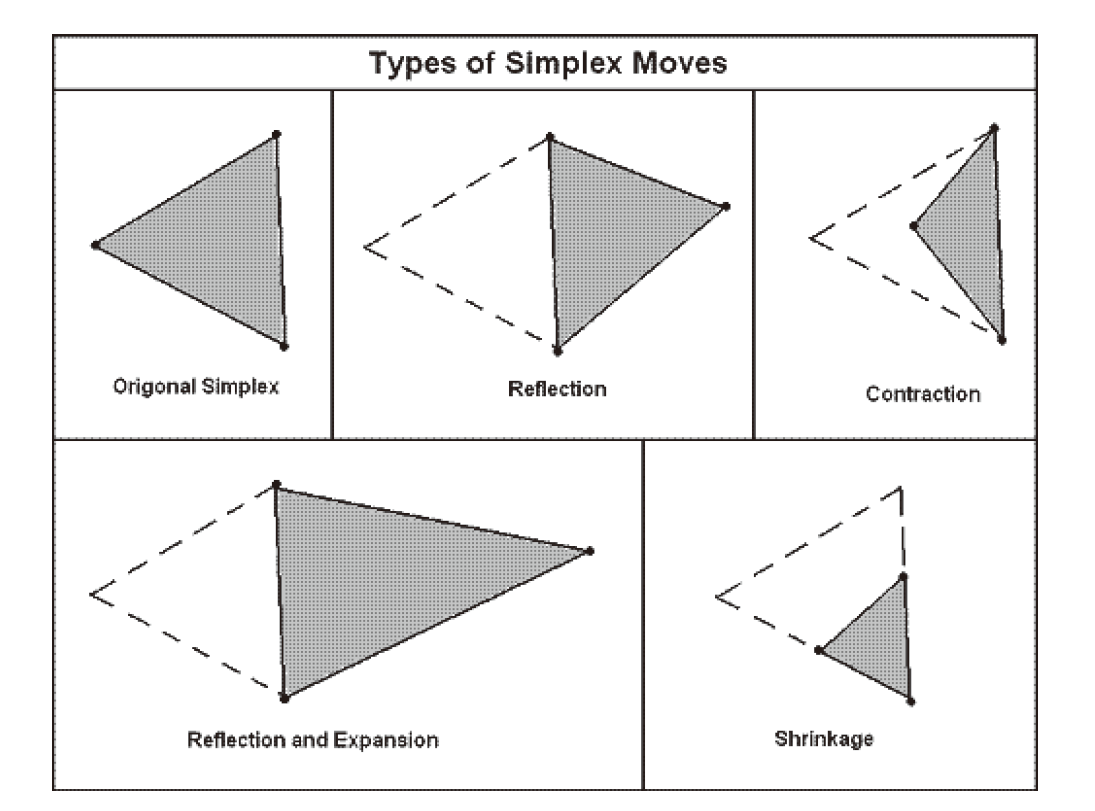
\includegraphics[width = 4.5in]{Nelder_Mead.png}
  \end{figure}
\end{frame}

\begin{frame}
\frametitle{Newton / Quasi-Newton Methods}
  \begin{itemize}
    \item[--] \textcolor{red}{Second-order} Taylor approximation of $f$ yields
    \[
      f\left(\mathbf{x}^{n+1}\right)\approx f\left(\mathbf{x}^{n}\right)+\nabla f\left(\mathbf{x}^{n}\right)'\left(\mathbf{x}^{n+1}-\mathbf{x}^{n}\right)+\frac{1}{2}\left(\mathbf{x}^{n+1}-\mathbf{x}^{n}\right)'H\left(\mathbf{x}^{n}\right)\left(\mathbf{x}^{n+1}-\mathbf{x}^{n}\right)
    \]
    \bigskip
    \item[--] Updating equation in $\mathbb{R}^n$
    \[
      \mathbf{x}^{n+1}=\mathbf{x}^{n}-H\left(\mathbf{x}^{n}\right)^{-1}\nabla f\left(\mathbf{x}^{n}\right)
    \]
    \bigskip
    \item[--] Using the updating rule, the Taylor approximation becomes
    \[
      f\left(\mathbf{x}^{n+1}\right)\approx f\left(\mathbf{x}^{n}\right)-\frac{1}{2}\left(\mathbf{x}^{n+1}-\mathbf{x}^{n}\right)'H\left(\mathbf{x}^{n}\right)\left(\mathbf{x}^{n+1}-\mathbf{x}^{n}\right)
    \]
    therefore as long as the Hessian is \textcolor{red}{approximated by a positive definite matrix}, the algorithm moves in the right direction
  \end{itemize}
\end{frame}

\begin{frame}
\frametitle{Newton / Quasi-Newton Methods}
  \begin{itemize}
    \item[--] Computation of Hessian is time consuming -- that's where quasi-Newton methods come handy
    \bigskip
    \item[--] Simplest option: set Hessian to $I$ then
    \[
      \mathbf{x}^{n+1}=\mathbf{x}^{n}-\nabla f\left(\mathbf{x}^{n}\right)
    \]
    this method is called \textcolor{red}{steepest descent}
    \bigskip
    \item[--] Berndt-Hall-Hall-Hausman (BHHH) method uses \textcolor{blue}{the outer product of the gradient vectors} to replace the Hessian
    \item[--] Broyden-Fletcher-Foldfarb-Shanno (BFGS) and Davidon-Fletcher-Powell (DFP) algorithms: \textcolor{blue}{secant methods that approximate Hessian with symmetric positive definite matrix}
  \end{itemize}
\end{frame}

\section{Numerical Integration}

\begin{frame}
\frametitle{Numerical Integration Methods}
  \begin{itemize}
    \item[--] We are interested in approximating
    \[
      \int_{a}^{b}f\left(x\right)\mathrm{d}x
    \]
    \bigskip
    \item[--] Three approaches to computing integral:
    \begin{itemize}
      \medskip
      \item[1.] \textcolor{red}{Newton-Cotes methods}: employ piecewise polynomial approximations to the integrand with evenly spaced nodes
      \medskip
      \item[2.] \textcolor{red}{Gaussian Quadrature}: choose nodes and weights efficiently such that they satisfy some moment-matching conditions
      \medskip
      \item[3.] \textcolor{red}{Monte-Carlo methods}: use equally weighted random nodes
    \end{itemize}
  \end{itemize}
\end{frame}

\begin{frame}
\frametitle{Newton-Cotes: Trapezoid rule}
  \begin{itemize}
    \item[--] Approximate $f$ with \textcolor{red}{piecewise linear} function
    \bigskip
    \item[--] Partition the interval $[a,b]$ into $n$ subintervals of equal length $h=(b-a)/n$ and endpoint nodes $x_{i}=a+ih$
    \bigskip
    \item[--] The area under the piecewise linear approximation for subinterval $i$ is
    \[
      \int_{x_{i}}^{x_{i+1}}f\left(x\right)\mathrm{d}x\approx\left[\frac{f\left(x_{i+1}\right)+f\left(x_{i}\right)}{2}\right]\cdot h
    \]
    and hence
    \[
      \int_{a}^{b}f\left(x\right)\mathrm{d}x\approx\sum_{i=0}^{N}\omega_{i}f\left(x_{i}\right)
    \]
    where $\omega_{i}=h$ for all $i$ unless $i=0,N$ where $\omega_{i}=h/2$
  \end{itemize}
\end{frame}

\begin{frame}
\frametitle{Newton-Cotes: Simpson rule}
  \begin{itemize}
    \item[--] Simpson rule based on \textcolor{red}{quadratic approximation} of the function
    \bigskip
    \item[--] Similar expression as trapezoid rule. Figure out what $\omega_{i}$ need to be
    \bigskip
    \item[--] If $f$ is smooth then Simpson rule is preferred because approximation error is square of Trapezoid rule error
    \bigskip
    \item[--] If $f$ is nondifferentiable at some points then trapezoid rule may be better
  \end{itemize}
\end{frame}

\begin{frame}
\frametitle{Gaussian Quadrature}
  \begin{itemize}
    \item[--] In general suppose you want to compute an integral of the type
    \[
      \int_{a}^{b}f\left(x\right)\omega\left(x\right)\mathrm{d}x\approx\sum_{i=1}^{n}\omega_{i}f\left(x_{i}\right)
    \]
    \bigskip
    \item[--] Choose the suitable quadrature

    \begin{table}
      \centering
      \begin{tabular}{cccc}
        \hline
        Range & $\omega\left(x\right)$ & Polynomial family  & Quadrature method\tabularnewline
        \hline
        $\left[-1,1\right]$ & $1$ & Legendre & Gauss-Legendre\tabularnewline
        $\left(-1,1\right)$ & $\sqrt{1-x^{2}}$ & Chebyshev & Gauss-Chebyshev\tabularnewline
        $\left(0,\infty\right)$ & $\exp\left(-x\right)$ & Laguerre & Gauss-Laguerre\tabularnewline
        $\left(-\infty,\infty\right)$ & $\exp\left(-x^{2}\right)$ & Hermite & Gauss-Hermite\tabularnewline
        \hline
      \end{tabular}
    \end{table}
  \end{itemize}
\end{frame}

\end{document}
